\documentclass[11pt]{article}
\usepackage[margin=1in]{geometry}          
\usepackage{graphicx}
\usepackage{amsthm, amsmath, amssymb}
\usepackage{setspace}\onehalfspacing
\usepackage[loose,nice]{units} %replace "nice" by "ugly" for units in upright fractions
\usepackage{longtable}
\usepackage{hyperref}
\usepackage{float}

%Import the natbib package and sets a bibliography styles
\usepackage{natbib}
%\bibliographystyle{abbrvnat}
\bibliographystyle{unsrt} %numbers references in the order they appear in the text
%\setcitestyle{authoryear}
\setcitestyle{numbers,square}

\title{Reference sheet for {\it yuki} version 2.2 usage}
%\author{Babak A. Ardekani, PhD}
%\date{Spring 2015}

\begin{document}
\maketitle
\noindent {\large \bf Introduction:} 
The computer program {\it yuki} is a part of the Automatic Registration Toolbox (ART) package 
developed by Dr. Babak A. Ardekani. It is designed to automatically segment the corpus callosum
(CC) mid-sagittal cross-sectional area from 3D T1-weighted structural MRI of the human brain.

%The {\it acpcdetect} program is a module of the Automatic Registration Toolbox (ART). 
%The program takes a 3D T1-weighted structural MRI of the human brain as input. 
%It automatically detects the mid-sagittal plane (MSP) using the method described in \citep{pmid9533596}.
%It then detects the AC and PC intersection points on the MSP using the method described in \citep{pmid19264138}. 
%Finally, it detects 8 additional landmarks (the so-called Orion landmarks) on the MSP using the method 
%described in \citep{pmid35288224}.  
%This information is used to tilt-correct the input volume into a standard orientation.  
%In this orientation: (1) the MSP is precisely aligned with the central plane of the FOV; 
%(2) the anterior-posterior (AP) axis is on the MSP and aligned with the AC-PC line; 
%(3) the inferior-superior (IS) axis is on the MSP and perpendicular to the AC-PC line; 
%(4) the left-right (LR) axis is perpendicular to the MSP; and 
%(5) the FOV center is approximately the mid-point between the AC and the PC on the MSP. 
%The FOV center can alternatively be placed on the AC point using the -center-AC option.  

\noindent {\large \bf Installation on Linux and MacOS systems:}
A video demonstration of installing ART software can be found
\href{https://www.youtube.com/watch?v=xCawMFQr50M\&t=26s}{\underline{here}}.
Although I made this video for installing {\it atra}, a different module of ART, 
the steps are similar.

To install {\it yuki}, you may need 
to be logged in as root, depending on the permissions of the directory in which
you are installing {\it yuki}. Let's assume that {\it yuki} will be installed in
/usr/local/art.
\begin{itemize}
\item[(a)] Set the ARTHOME environment variable to /usr/local/art. If ARTHOME is already
defined on your system, then you can skip this step. Otherwise, ``sh'' or ``bash'' 
users may define ARTHOME using the following command: 

export ARTHOME=/usr/local/art 

To do this automatically at login, users should add the above line to their 
``.bashrc'' or ``.profile'' file. 
Users of ``csh'' or ``tcsh'' may use the following command:

setenv ARTHOME /usr/local/art 

and add it to their ``.cshrc'' or ``.tcshrc'' file.

\item[(b)] Download the Linux or MacOS version of the software from 
\href{https://www.nitrc.org/projects/art}{https://www.nitrc.org/projects/art}.
and move it to \$ARTHOME.

\item[(c)] Unpack the package:

cd \$ARTHOME

tar -xvzf yuki2.2*.tar.gz

\item[(d)] Add the directory \$ARTHOME/bin to your PATH. This can be done by executing the
following command and adding it to the ``.bashrc'' file:

export PATH=\$ARTHOME/bin:\$PATH

\end{itemize}

\noindent {\large \bf Usage:} 

yuki [options] -i \textless input-filename\textgreater.nii

\noindent {\large \bf Required argument:}

\begin{longtable}{p{0.25\textwidth}p{0.68\textwidth}}
-i \textless input-filename\textgreater.nii &
3D T1-weighted MRI brain volume in NIFTI format of type short or unsigned short.
This is the structural MRI volume on which we would like to segment the CC.
\end{longtable}

\noindent {\large \bf Options:}

\begin{longtable}{p{0.25\textwidth}p{0.68\textwidth}}
-verbose (-v) & Enables verbose mode \\

-version (-V) &
	Reports software version \\

-help (-h) &
	Prints help message \\

-o \textless output-prefix\textgreater & 
	Prefix for naming output files (default = \textless input-filename\textgreater) \\

-n \textless integer\textgreater & Specifies the number of atlases to be used 
(default = 49 ).\\

-csv \textless csvfile\textgreater.csv & CC measurements (area, perimeter, etc.) will be 
appended to this file in comma-separated values (CSV) format 
(default = \textless output-prefix\textgreater.csv) \\

-Hampel (-H) & When this option is selected, the program subdivides the CC area
according to the Hampel et al.\ \citep{Hampel1998-fz} method. The 5 sub-areas are stored
in the output CSV file. The sub-areas are visualized in the PPM format image
\textless output-prefix\textgreater\_cc\_hampel.ppm
(Fig.\ \ref{fig:hampel}) and also saved in the NIFTI file
\textless output-prefix\textgreater\_cc\_hampel.nii.\\

-Witelson (-W) & When this option is selected, the program subdivides the CC area
according to the Witelson et al.\ \citep{Narayan2016-es} method. The 7 sub-areas are stored
in the output CSV file. The sub-areas are visualized in the PPM format image
\textless output-prefix\textgreater\_cc\_witelson.ppm
(Fig.\ \ref{fig:witelson}) and also saved in the NIFTI file
\textless output-prefix\textgreater\_cc\_witenson.nii.\\

-png & Outputs *.png images in addition to the *.ppm images \\

-lm \textless landmarks-file\textgreater &
A text file containing manually determined $(i, j, k)$ coordinates
of the AC, PC and VSPS (vertex of the superior pontine sulcus) landmarks in that order. 
When this file is supplied,
automatic detection of these landmarks is suppressed. This is useful
in cases when automatic landmark detection fails.
We recommend using the AFNI software for manual identification of these landmarks.
A video instruction for this can be found
\href{https://www.youtube.com/watch?v=q5GBaNnjOa8}{\underline{here}}.
\\

-A \textless filename.txt\textgreater & Uses a preselected set of atlases specified in 
``filename.txt'' instead of automated atlas selection. 
``filename.txt'' is always the output of a previous {\it yuki} run, namely
the output file
``*\_A.txt''. \\ 

-cc \textless corrected\_cc.nii\textgreater & This option is used when the out binary CC 
image is corrected manually and we need to recalculate the CC related measurements 
(area, circularity, etc.) for the corrected image.  Typically, when there is an error
in ``output-prefix\_cc.nii'', we load the
``output-prefix\_msp.nii'' in ITK-SNAP and overlay
``output-prefix\_cc.nii'' as a segmentation.  The segmentation
is manually corrected and saved under a different filename, for example,
``output-prefix\_corrected\_cc.nii''.  Then we run 
``yuki -cc output-prefix\_corrected\_cc.nii'' to obtain the corrected CC measurements.
\\ 

-T \textless filename.mrx\textgreater & Applies the transformation matrix in 
``filename.mrx'' to reorient the subject volume in preperation for CC detection. 
This option disables automatic reorientation. The format of ``filename.mrx'' is 
the same as the ``output-prefix\_msp.mrx'' transformation matrix.\\

\end{longtable}

\begin{figure}[t!]
\begin{center}
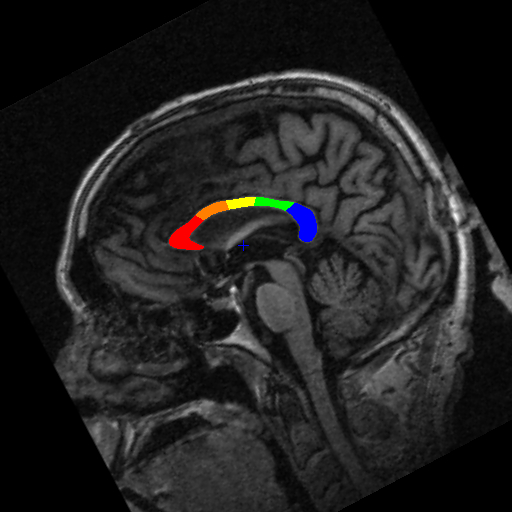
\includegraphics[scale=.5]{v1_cc_hampel.jpg}
\caption{Five automatically detected CC sub-divisions as defined by Hampel et al.\ 
\citep{Hampel1998-fz}.
}
\label{fig:hampel}
\end{center}
\end{figure}

\begin{figure}[H]
\begin{center}
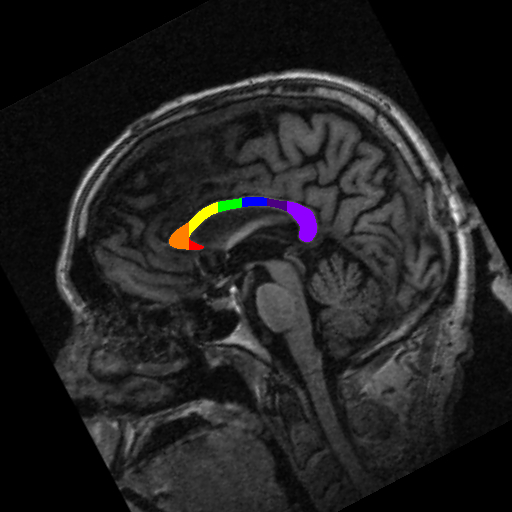
\includegraphics[scale=.5]{v1_cc_witelson.jpg}
\caption{Seven automatically detected CC sub-divisions as defined by Witelson et al.\ 
\citep{Narayan2016-es}.
}
\label{fig:witelson}
\end{center}
\end{figure}

\noindent {\large \bf Output files:}

\noindent We will describe the program outputs after the following command:

yuki -i v1.nii -v -o op -H -W \\
Here the input image is ``v1.nii'', the output prefix is chosen as ``op'' and the
program is asked to further subdivide the CC using both the Hampel (-H) and Witelson (-W)
methods.

\begin{longtable}{p{0.4\textwidth}p{0.53\textwidth}}
op.csv & CC measurements (area, perimeter, etc.) will be 
appended to this file in comma-separated values (CSV) format.
The following measurements are stored: input volume, CC area (mm${}^2$), 
CC perimeter (mm), CC circularity (unitless),
CC length (mm), W1--W7 (Witelson sub-areas in mm${}^2$), 
and C1--C5 (Hampel sub-areas in mm${}^2$). \\

v1\_ACPC\_sagittal.ppm &
	Sagittal view of the detected AC/PC locations in
	PPM format (Fig.\ \ref{fig:sagittal}) \\

v1\_ACPC\_axial.ppm &
	Axial view of the detected AC/PC locations in PPM
	format (Fig.\ \ref{fig:axial}) \\

v1\_orion.ppm &
	Mid-sagittal view of the detected Orion landmarks in
	PPM format (Fig.\ \ref{fig:orion}).
	The method for detecting these landmarks is described in \citep{pmid35288224}. \\

v1\_orion.txt &
	Stores $(i, j, k)$ coordinates of the 8 detected Orion landmarks \\

v1\_ACPC.txt &
	Stores the detected AC, PC and VSPS $(i, j, k)$ coordinates.
	The equation of the automatically detected MSP is also saved in this file. \\

op\_msp.mrx & A rigid-body linear transformation matrix (in ART format) that
would transform the input image (v1.nii) to a tilt-corrected Posterior-Inferior-Left (PIL) 
orientation.  Detailed information about how this matrix is obtained 
is given in \citep{pmid35288224}.\\

op\_msp.nii &  A single slice NIFTI mid-sagittal plane (MSP) image obtained by 
applying op\_msp.mrx to v1.nii. This is the image on which the CC is segmented.  \\

op\_cc.nii &  A single slice binary NIFTI image representing the segmented whole CC
on op\_msp.nii. \\

op\_cc.ppm &  A PPM image in op\_msp.nii orientation showing the results of CC
segmentation.  CC perimeter is indicated in yellow and cyan.  An estimated medial axis
is indicated in red.  Some automatically detected landmarks are indicated by blue the
+ signs. An example is shown in Fig.\ \ref{fig:op}.
\\

op\_cc\_hampel.ppm & PPM format image aligned with op\_msp.nii and op\_cc.nii,
output with -H option. The program subdivides the CC area 
according to the Hampel et al.\ \citep{Hampel1998-fz} method. 
The 5 sub-areas are stored
in the output CSV file. The sub-areas are visualized in this image 
(see Fig.\ \ref{fig:hampel}). \\ 

op\_cc\_hampel.nii & NIFTI format version of op\_cc\_hampel.ppm output with -H option. 
The 5 sub-divisions are labeled from 1 to 5. \\

op\_cc\_witelson.ppm & PPM format image aligned with op\_msp.nii and op\_cc.nii,
output with -W option. The program subdivides the CC area 
according to the Witelson et al.\ \citep{Narayan2016-es} method. 
The 7 sub-areas are stored
in the output CSV file. The sub-areas are visualized in this image 
(see Fig.\ \ref{fig:witelson}). \\ 

op\_cc\_witelson.nii & NIFTI format version of op\_cc\_witelson.ppm output with -W option. 
The 7 sub-divisions are labeled from 1 to 7. \\

op\_A.txt &  The list of automatically selected atlases.  
The default number of atlases is 49.  This number
can be changed using the -n option.  The first line in the op\_A.txt file indicates the
number of atlases used.  The subsequent lines indicate the indices of the automatically selected
atlas.  The last line indicates a threshold used for label fusion for obtaining the final 
CC segmentation.  This file may be used later as an optional {\em input} to {\it yuki} 
to override the automatic atlas selection and label fusion threshold selection on a subsequent
analysis.
\\

op\_TP.txt & After CC segmentation, {\it yuki} attempts to measure the CC thickness profile.
The estimated profile is stored in this file.  This part of the program is a work in progress,
and the output profile is sometimes not accurate.  The op\_cc.ppm image should be inspected
to ensure that the CC medial axis is correctly detected.  If so, then the thickness profile
may be relied upon.  op\_TP.txt contains 101 numbers representing lengths (mm) of 99 line
segments perpendicular to the medial axis along the length of the CC. \\

\end{longtable}

\begin{figure}[t!]
\begin{center}
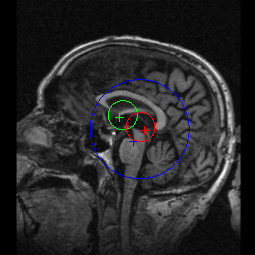
\includegraphics[scale=1.0]{v1_ACPC_sagittal.jpg}
\caption{v1\_ACPC\_sagittal.ppm shows the automatically detected MSP, the AC (green +), 
the PC (red +) and the VSPS (blue +).  
}
\label{fig:sagittal}
\end{center}
\end{figure}
\begin{figure}[H]
\begin{center}
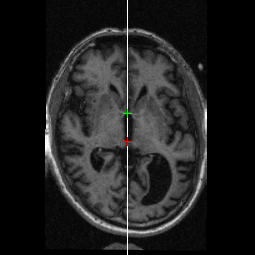
\includegraphics[scale=1.0]{v1_ACPC_axial.jpg}
\caption{v1\_ACPC\_axial.ppm shows the automatically detected MSP, the AC (green +), 
the PC (red +).
}
\label{fig:axial}
\end{center}
\end{figure}
\begin{figure}[H]
\begin{center}
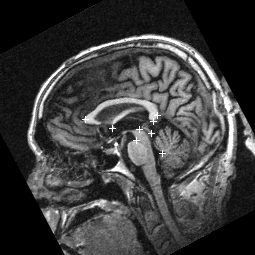
\includegraphics[scale=1.0]{v1_orion.jpg}
\caption{v1\_orion.ppm shows the 8 automatically detected
Orion landmarks on the pitch-corrected MSP.
}
\label{fig:orion}
\end{center}
\end{figure}
\begin{figure}[H]
\begin{center}
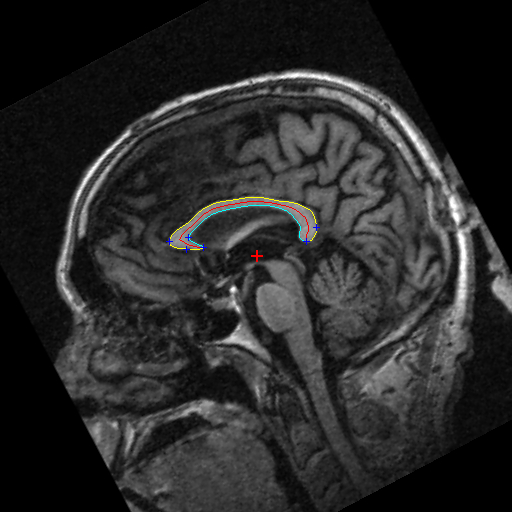
\includegraphics[scale=.5]{op_cc.jpg}
\caption{
A PPM image in op\_msp.nii orientation showing the results of CC
segmentation.  
}
\label{fig:op}
\end{center}
\end{figure}

\noindent {\large \bf Failure in landmark detection:} 
It is strongly recommended that the *ppm images be inspected to ensure that 
the automatic MSP, AC, PC and VSPS detections were successful.  
If there is a failure in this process, the AC, PC and VSPS landmarks should be
manually supplied to the program  using the -lm argument. 
We recommend
using the AFNI software for manual identification of these landmarks. 
A video instruction for this can be found 
\href{https://www.youtube.com/watch?v=q5GBaNnjOa8}{\underline{here}}.

\bibliography{references}

\end{document}
